\documentclass{article}
\usepackage[utf8]{inputenc}
\usepackage{geometry}
 \geometry{
 a4paper,
 total={170mm,257mm},
 left=20mm,
 top=20mm,
 }
\usepackage{polski}
\usepackage{natbib}
\usepackage[capbesideposition=right]{floatrow}
\usepackage{graphicx}
\usepackage{pbox}
\usepackage{float}
\usepackage[dvipsnames]{xcolor}
\usepackage{caption}
\usepackage{wrapfig}
\usepackage{graphicx}
\usepackage{tikz}
    \usetikzlibrary{
        arrows,
        shadows,
        shapes,
        automata,
        positioning,
        arrows.meta
    }
\usepackage{pgfplots}
\usepackage{tabularx}
\usepackage{booktabs}
\usepackage{amsfonts}
\pgfplotsset{compat=1.17}

\title{CCG Simulation}
\author{Piotr Jasik, Damian Zimon}
\begin{document}

\maketitle

\clearpage

\section{Analysis of simulation}
In this agent simulation we'll be examining flow of a two player card game. Players will play cards to gain \textbf{Strength} advantage over the opponent. To simplify the simulation, players will be playing cards in a random manner. Cards will be put into the play on the table where they will be interacting with each other.

\begin{enumerate}
    \item Card behaviors:
    \begin{itemize}
        \item Each card played influences your opponent's next played card.
        \item Allied cards may empower each other, gaining higher Strength when played together, compared to playing the same cards independently.
    \end{itemize}
    \item Simulation \textcolor{red}{parameters}:
    \begin{itemize}
        \item Number of played rounds
        \item Point advantage needed to end the game
        \item Number of cards in each player's deck
        \item Pool of available cards
        \item Balance of the cards
        \item Card hand size
    \end{itemize}
\end{enumerate}

\section{Rules of the game}

    The main objective of the game is to achieve the highest possible \textbf{Strength} score. 
    Player begin the game by drawing \textcolor{red}{5} cards from their deck.
    At the beginning of a turn, players draw a card from their deck.
    Players take turns playing one card each.
    Played card adds it's \textbf{Strength} value to the corresponding player's score. 
    In addition, cards interact with each other e.g. by boosting \textit{Attributes} or by manipulating \textbf{Strength} score. 
    The game has 2 end conditions: 
    
    \begin{enumerate}
        \item After \textcolor{red}{10} rounds.
        \item Player accumulates a lead of \textcolor{red}{50} points over the other player.
        \item Player runs out of cards to play.
    \end{enumerate}
    
    \begin{flushleft}
        Whenever an end condition is triggered, the round current round is resolved, and then the game ends. The player with the highest score is considered a winner.
    \end{flushleft}

\section{Rules of deck creation}
    
    Each player starts the game with his own deck of \textcolor{red}{30} cards. 
    The cards can be selected from a pool of \textcolor{red}{100} cards.

\section{Rules of pool generation}
    
    The pool, from which the decks will be created, consist of \textcolor{red}{100} cards and have randomly generated properties.

\subsection{Power Level of a card}
    
    Cards begin with randomly generated card Power Level value.  Whenever a property 
    is assigned to a card, it is then subtracted from the card Power Level value. 
    This value can never be negative. The balance of the game, which can be set before the simulation to any integer between 0 and 5, determines the upper and lower bound from which the Power Level value is generated:
    
    \begin{center}
        $Power Level = 25\pm \textcolor{red}{Balance}$ \\
    \end{center}

\subsection{Card Properties}

\subsubsection{Card \textbf{Strength}}

    First property of each card is it's \textbf{Strength}. It's the main factor when calculating \textbf{Strength} score. Other properties may further manipulate it's value - usually by decreasing your opponent's card's \textbf{Strength}, while increasing your own. \textbf{Strength} value is randomly generated, assuming values shown below, with one digit of precision.

\begin{center}
   $1 \leq \textbf{Strength} \leq 10$   
\end{center}
  
\subsubsection{Card \textit{Attributes}}

    Second property of each card are it's \textit{Attribute} values. Main purpose of \textit{Attributes} is to introduce direct interaction between two cards. Each \textit{Attribute} value is generated independently in following range: 
    
    \begin{center}
    $0 \leq \textit{Attribute} \leq 5, \textit{Attribute} \in \mathbb{Z}$
    \end{center}
    
    \begin{flushleft}
        Each card has 3 \textit{Attributes}: 
    \end{flushleft}
    
    \begin{itemize}
        \item \textcolor{RoyalBlue}{Water}
        \item \textcolor{BrickRed}{Fire}
        \item \textcolor{OliveGreen}{Nature}
    \end{itemize}
    
    \begin{flushleft}
        Whenever a card is played (except for first \& last card played in the game), it's \textbf{Strength} is reduced according to this formula(Player A played 1st, then Player B):
    \end{flushleft}
    
    \begin{center}
        $\frac{\textcolor{RoyalBlue}{Water A} * \textcolor{BrickRed}{Fire B} + \textcolor{BrickRed}{Fire A} * \textcolor{OliveGreen}{Nature B} + 
        \textcolor{OliveGreen}{Nature A} * \textcolor{RoyalBlue}{Water B}}{100}*\textbf{Strength} B$
    \end{center}
    
    \begin{flushleft}
        Example: 
    \end{flushleft}
    
    \begin{center}
    \begin{tabular}{|c|c|c|}
    \hline
        Property & Card A & Card B  \\
    \hline
        \textbf{Strength} & 4.7 & 7.8 \\
    \hline
        \textcolor{RoyalBlue}{Water} & 4 & 3 \\
    \hline
        \textcolor{BrickRed}{Fire} & 3 & 0 \\
    \hline
        \textcolor{OliveGreen}{Nature} & 5 & 1 \\
    \hline
    \end{tabular}
    \begin{tabular}{c}
    $\frac{\textcolor{RoyalBlue}{4} * \textcolor{BrickRed}{0} + \textcolor{BrickRed}{3} * \textcolor{OliveGreen}{1} + 
    \textcolor{OliveGreen}{5} * \textcolor{RoyalBlue}{3}}{100}*7.8 = 1.4$\\ \\ $7.8 - 1.4 = 6.4$
    \end{tabular}
    \end{center}
    \begin{flushleft}
    The \textbf{Strength} of Card B will be changed to 6.4.
    \end{flushleft}
    
\subsubsection{Card Traits}

    The last property of a card are Traits. It's a predefined list of additional effects that impact the course of the game. Each Trait has a Power Level cost, which corresponds to how much of Power Level is decreased from a card in the process of card generation. 
    
\begin{table}[h]
    \noindent\makebox[\textwidth]{\begin{tabular}{| c | c | l | c |}
        \hline
        Cost & Name & Effect & Symbol\\ \hline
        15 & \textit{Swift} & You may play second card this round. & $>>$ \\  \hline
        11 & \textit{Symbiotic} & Double the \textbf{Strength} of your next card with this trait. & $\star$ \\ \hline
        7 & \textit{Poisonous} &\pbox{25cm}{If you control 3 cards with this trait, 
        \\destroy random card played by your opponent.}  & $\dagger$ \\  \hline
        4 & \textit{Empowering} & Your next card's \textit{Attributes} are increased by 1 each. & +\\ \hline
        3 & \textit{Sabotaging} & Your opponent's next card loses random \textit{Attribute} (set it to 0.) & $\downarrow$ \\ \hline
        2 & \textit{Supporting} & Your next card \textbf{Strength} is increased by 1.& $\uparrow$ \\ \hline
    \end{tabular}}
    
\end{table}

\clearpage

\subsection{Example of a single card generation}

\vspace{2cm}

\centering

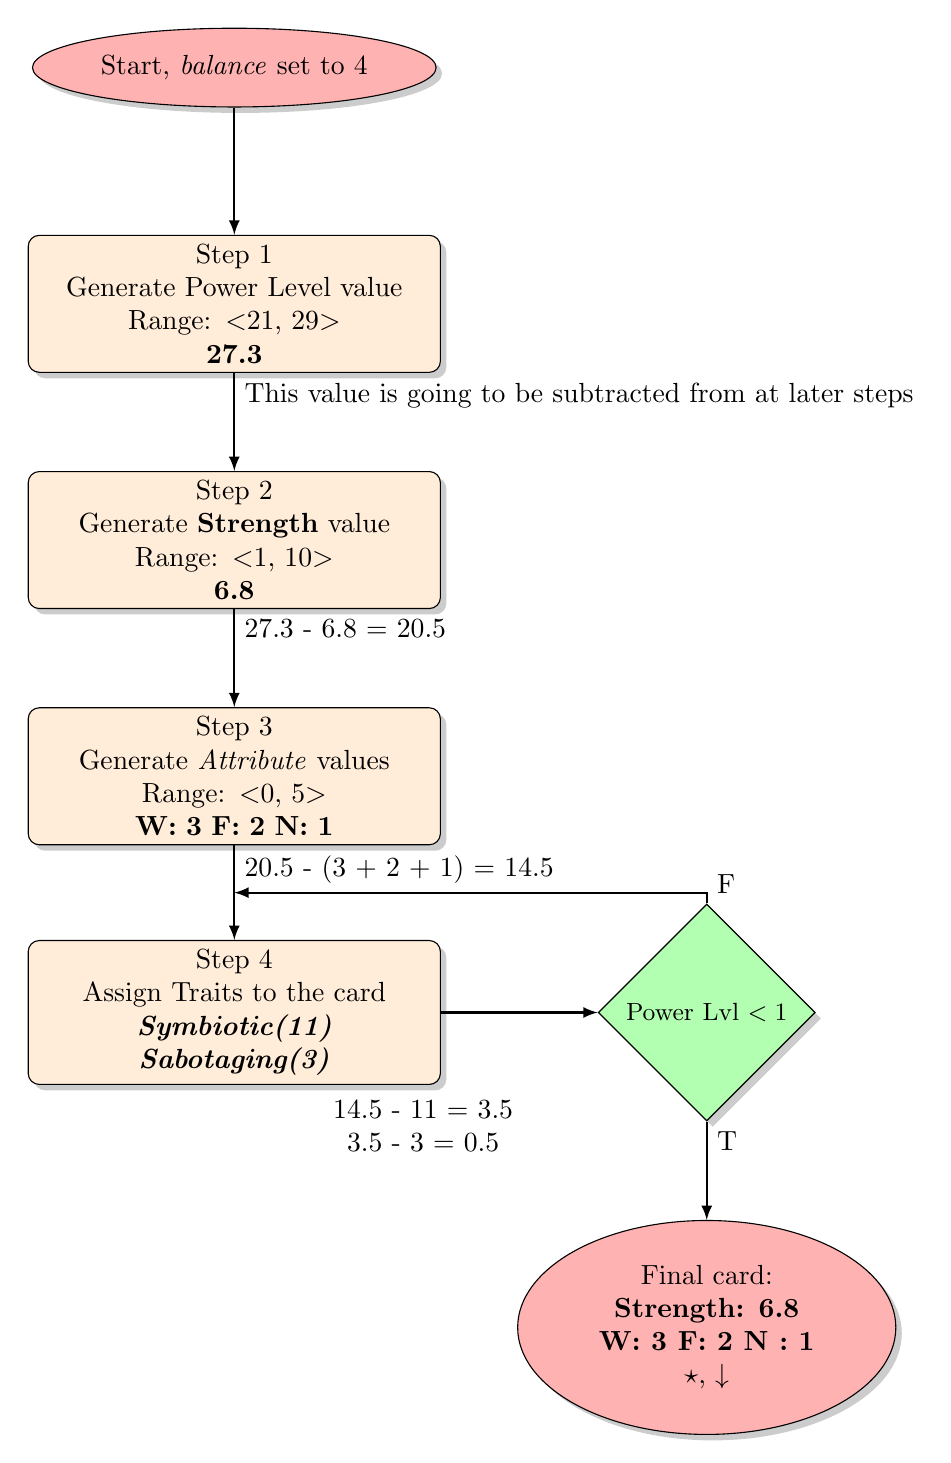
\begin{tikzpicture}
[baseshape/.style={minimum width=3.5cm, minimum height=1cm,text centered, font=\normalsize,draw=black, drop shadow=black!40},
startstop/.style={baseshape, ellipse, fill=red!30},
io/.style={baseshape, trapezium, trapezium stretches=true, 
trapezium left angle=70, trapezium right angle=110, fill=blue!30},
process/.style={baseshape, rectangle, rounded corners, text width=5cm, fill=orange!15},
decision/.style={baseshape, diamond, minimum width=1cm, fill=green!30},
arrow/.style={thick, -latex},
node distance=3cm,]
    \node (step0) [startstop] {Start, \textit{balance} set to 4}; 
    \node (step1) [process, below of=step0] {Step 1 \\ Generate Power Level value \\ Range: $<$21, 29$>$ \\ \textbf{27.3}};
    \node (step2) [process, below of=step1] {Step 2 \\ Generate \textbf{Strength} value \\ Range: $<$1, 10$>$\\ \textbf{6.8}};
    \node (step3) [process, below of=step2] {Step 3 \\ Generate \textit{Attribute} values \\ Range: $<$0, 5$>$ \\ \textbf{W: 3 F: 2 N: 1}};
    \node (step4) [process, below of=step3, label=below right:{\begin{tabular}{c}
         14.5 - 11 $=$ 3.5  \\ 3.5 - 3 $=$ 0.5
    \end{tabular} }] {Step 4 \\ Assign Traits to the card \\ \textit{\textbf{Symbiotic(11) Sabotaging(3)}}};
    \node (step5)[decision, right of=step4, xshift = 3cm] {\small{Power Lvl }$ < 1$};
    \node (step6) [startstop, below of=step5, yshift = -1cm] {
    \begin{tabular}{c}
         Final card:  \\
         \textbf{\textbf{Strength}: 6.8} \\
         \textbf{W: 3 F: 2 N : 1} \\
         $\star$,  $\downarrow$
    \end{tabular}};
    \draw[arrow] (step0) -- (step1);
    \draw[arrow] (step1) -- node[at start, anchor=north west]{This value is going to be subtracted from at later steps}(step2);
    \draw[arrow] (step2) -- node[at start, anchor=north west]{27.3 - 6.8 = 20.5}(step3);
    \draw[arrow] (step3) -- node[at start, anchor=north west]{20.5 - (3 + 2 + 1) = 14.5} coordinate(a)(step4);
    \draw[arrow] (step4) -- (step5);
    \draw[arrow] (step5) |- node[at start, anchor=south west]{F}(a);
    \draw[arrow] (step5) -- node[at start, anchor=north west] {T} (step6);
\end{tikzpicture}

\clearpage

\end{document}
